% 8.1 “수렴”과 “정답”의 분리(명시)
% 8.2 비식별/약식별에서 supervised 학습의 최적해가 왜 평균화되는가(당신들이 이미 가진 이론 전개 배치)
% 8.3 OGTT: SI·σ 협곡( (SI\cdot\sigma=C) )과 라벨 혼재 → 평균으로 붕괴
% 8.4 결론: 이 문제는 “네트워크가 못해서”가 아니라 “관측 정보가 부족해서” 발생

\section{Correctness: what fixed point does supervised learning select?}
\label{sec:correctness}

While Sections~\ref{sec:method}--\ref{sec:convergence} guarantees that the fixed-point iteration $\theta^{(k+1)} = T(\theta^{(k)};\mathbf{x}_\mathrm{obs})$ converges to a unique fixed point $\theta^*$, a fundamental question remains: 
\emph{Does the resulting fixed point $\theta^*$ correspond to the ground-truth parameter $\theta^\mathrm{true}$?}
We demonstrate that our teacher-forced supervised learning objective explicitly minimizes the one-step residual, forcing the network's fixed point to align with the ground truth in structurally identifiable regimes.

\subsection{Correctness is controlled by a one-step residual}
\label{subsec:correctness-residual}

Let $\theta_{\mathrm{true}}$ denote the ground-truth parameter corresponding to a given observation feature $\mathbf{u}$,
and define the one-step residual
\[
\varepsilon(\mathbf{u}) := \|T(\theta_{\mathrm{true}};\mathbf{u})-\theta_{\mathrm{true}}\|_2.
\]
As summarized in Remark~\ref{rem:approx-fp}, if $T(\cdot;\mathbf{u})$ is a contraction with constant $K<1$, then the fixed point $\theta^\star(\mathbf{u})$
satisfies the stability bound
\[
\|\theta^\star(\mathbf{u})-\theta_{\mathrm{true}}\|_2 \le \frac{\varepsilon(\mathbf{u})}{1-K}.
\]
Therefore, even when convergence is guaranteed, accurate recovery requires that the learning procedure makes $\varepsilon(\mathbf{u})$ small
for typical inputs $\mathbf{u}$.

\subsection{What the teacher-forced supervised objective encourages}
\label{subsec:correctness-supervised}

Recall that the networks $H_\phi$ and $P_\psi$ are trained with teacher forcing using supervised MSE losses.
Intuitively, if the hidden-state estimator approximates the conditional mapping
$H_\phi(\mathbf{u},\theta_{\mathrm{true}})\approx \mathbf{x}_{\mathrm{hid}}$
and the parameter estimator approximates
$P_\psi(\mathbf{u},\mathbf{x}_{\mathrm{hid}})\approx \theta_{\mathrm{true}}$,
then the composition $T(\theta;\mathbf{u}) = P_\psi(\mathbf{u},H_\phi(\mathbf{u},\theta))$ approximately preserves the ground-truth parameter,
i.e., $T(\theta_{\mathrm{true}};\mathbf{u})\approx\theta_{\mathrm{true}}$.
This motivates the use of teacher-forced supervised training as a means to reduce $\varepsilon(\mathbf{u})$.

However, this mechanism can break down when the inverse mapping from observations to parameters is not injective under the given observation scheme,
as is the case for glucose-only OGTT parameter estimation.

\subsection{OGTT: glucose-only observations and a non-identifiability valley}
\label{subsec:correctness-ogtt-valley}

Empirically, we observe that optimizing parameters using glucose-only information can produce a pronounced valley in the loss landscape:
different parameter pairs $(S_I,\sigma)$ yield nearly indistinguishable glucose trajectories.

\begin{figure}[t]
    \centering
    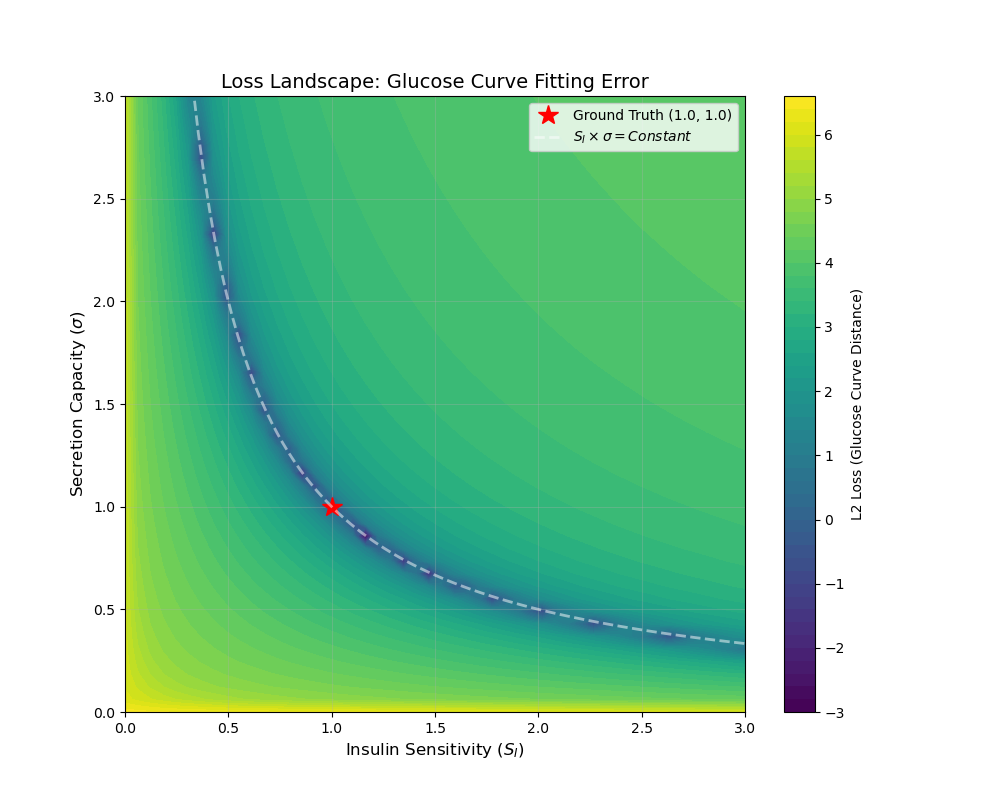
\includegraphics[width=0.78\linewidth]{figures/ogtt_loss_landscape.png}
    \caption{OGTT glucose-only loss landscape in the $(S_I,\sigma)$ plane.
    A pronounced valley indicates that multiple parameter pairs yield nearly indistinguishable glucose trajectories.
    In particular, near-optimal solutions concentrate along curves of approximately constant product $S_I\sigma\approx c$,
    suggesting weak identifiability under glucose-only observations.}
    \label{fig:ogtt-loss-landscape}
\end{figure}

A representative phenomenon is that near-optimal solutions concentrate along curves of the form $S_I\sigma \approx c$ for some constant $c$
depending on the trajectory.
In such a regime, a dataset may contain multiple distinct parameter labels that are consistent with essentially the same observed glucose features.
As a result, even in the population limit, mapping glucose-only features to a unique parameter pair can be ill-posed.

\subsection{Regression-to-mean under MSE and model collapse}
\label{subsec:correctness-mean}

We formalize the above intuition using a standard property of squared-loss regression.

\begin{proposition}[Squared-loss regression yields a conditional mean]\cite{bishop2006prml,hastie2009esl}
\label{prop:cond-mean}
Let $(\mathbf{u},\theta)$ be random variables with $\mathbb{E}\|\theta\|_2^2<\infty$.
Among all measurable functions $g(\mathbf{u})$ minimizing the risk
$
\mathbb{E}\big[\|\theta-g(\mathbf{u})\|_2^2\big],
$
an optimal solution is given by $g^\star(\mathbf{u})=\mathbb{E}[\theta\mid \mathbf{u}]$ (a.s.).
\end{proposition}

\begin{proof}
Fix $\mathbf{u}$ and minimize $\mathbb{E}[\|\theta-g\|_2^2\mid \mathbf{u}]$ over $g\in\mathbb{R}^p$.
Expanding the square shows the unique minimizer is the conditional mean.
\end{proof}

In the OGTT setting, $\mathbf{u}$ is constructed from glucose-only observations (and their derivative features).
When $(S_I,\sigma)$ is not uniquely determined by glucose, the conditional distribution $\theta\mid\mathbf{u}$ can be broad and multimodal.
Consequently, the conditional-mean predictor $\mathbb{E}[\theta\mid\mathbf{u}]$ may lie in the interior of the non-identifiability valley
(e.g., near a ``mean'' point on the curve $S_I\sigma\approx c$) rather than recovering the ground-truth pair.

This provides a principled explanation for the model-collapse behavior observed in our experiments:
the learned predictions concentrate on a low-dimensional set that does not match the true joint distribution of $(S_I,\sigma)$,
even when marginal or projected metrics appear accurate.

This observation also highlights a potential pitfall in evaluation:
metrics computed on individual parameter coordinates (or other low-dimensional projections) can appear favorable even when the predicted \emph{joint}
distribution over $(S_I,\sigma)$ is severely distorted.
For this reason, in Section~\ref{sec:experiments} we complement coordinate-wise errors with (i) joint-distribution diagnostics (e.g., scatter plots of
predicted vs.\ true pairs) and (ii) loss-landscape visualizations such as Figure~\ref{fig:ogtt-loss-landscape}.

\subsection{Takeaway}
\label{subsec:correctness-takeaway}

In summary, contractive fixed-point inference guarantees stable and efficient convergence (Section~\ref{sec:convergence}),
but correctness depends on whether the supervised learning signal can make $T(\theta_{\mathrm{true}};\mathbf{u})\approx \theta_{\mathrm{true}}$.
For OGTT with glucose-only observations, structural or practical non-identifiability leads to label ambiguity, and MSE training selects a conditional-mean
solution that can be far from any individual ground truth.
This limitation is inherent to the observation scheme and motivates additional information or priors, which we discuss in Section~\ref{sec:discussion}.